%%% Sekce – Správa nákupního košíku
%%%%% Wording: ⏳
%%%%% Styling: ⏳
%%%%% References: ⏳
%%% --------------------------------------------------------------
\section{Správa košíku}
\label{sec:implementace-kosik}
Druhou hlavní funkcí naší aplikace je správa košíku.
Tato komponenta umožňuje uživatelům přidávat, odebírat nebo vyměňovat vstupenky, které si vybrali z mapy sedadel, a slouží jako most mezi interaktivní mapou sedadel a procesem rezervace a platby.
Správa košíku je pro aplikaci klíčová, protože ovládá tok dat od výběru sedadel po proces rezervace a platby.

%%% Podsekce – Kontext košíku
%%%%% Wording: ⏳
%%%%% Styling: ⏳
%%%%% References: ⏳
%%% --------------------------------------------------------------
\subsection{Kontext košíku}
\label{subsec:implementace-kosik-kontext}
State košíku je spravován globálně v celé aplikaci pomocí React kontextu.
Definovali jsme \texttt{CartContext}, který obaluje celou aplikaci a poskytuje kontext pro přístup a manipulaci se stavem košíku.
CartContext je ve skutečnosti pouze poskytovatelem komponent, který obaluje aplikaci a poskytuje stav a akce košíku zbytku aplikace.
Hlavní logika se odehrává v použití hooku košíku, který vytváří instanci nákupního košíku, která zajišťuje stav a akce košíku.

%%% Podsekce – State a funkce košíku
%%%%% Wording: ⏳
%%%%% Styling: ⏳
%%%%% References: ⏳
%%% --------------------------------------------------------------
\subsection{State a funkce košíku}
\label{subsec:implementace-kosik-state}
Z pohledu vstupenek a sedadel košík uchovává hlavně vstupenky, které jsou přidány do košíku.
Tento stav je reprezentován polem objektů ve tvaru následujícího rozhraní:

\begin{minted}{typescript}
/**
 * CartedTicket type
 * @export
 */
export type CartedTicket = {
	/** unique carted ticket id */
	cartedTicketId: UUID;
	/** reference to the ticket received from API */
	ticket: VenueApiTypes.Ticket;
	/** reference to the specific seat */
	/** the Seat type received from API is extended with a specific category */
	/** also tickets array from the seat type is ommited as it does not make sense here */
	seat?: Extend<
		{
			category: VenueApiTypes.Category;
		},
		Omit<VenueApiTypes.Seat, 'tickets'>
	>;
};
\end{minted}

Košík, jak již bylo zmíněno, zpracovává různé akce, které lze na košíku provést.
Tyto akce, reprezentované jako handlery, zahrnují \texttt{addToCartHandler}, \texttt{removeFromCartHandler} a \texttt{replaceCartedTicketHandler}.
Také poskytuje metodu \texttt{getCartedTicketPrice}, která vrací cenu vstupenky v košíku na základě sedadla a kategorie vstupenky, protože cena vstupenky je definována kombinací její kategorie a vybraného sedadla.
Implementace metody \texttt{getCartedTicketPrice} je uvedena v následujícím ukázce kódu:

\begin{minted}{typescript}
/** returns carted ticket price */
const getCartedTicketPrice = (cartedTicket: Types.CartedTicket) => {
	/** ticket without seat */
	if (!isDefined(cartedTicket.seat)) return cartedTicket.ticket.price;
	/** get ticket category */
	const ticketCategory = valOrThrow(
		cartedTicket.ticket.categories.find(({ categoryId }) => categoryId === cartedTicket.seat?.categoryId),
		`Ticket category not found for seat ${cartedTicket.seat.seatId}`,
	);
	/** return ticket category price */
	return ticketCategory.price;
};
\end{minted}

Posledně košík uchovává memoizovanou hodnotu celkové ceny všech vstupenek v košíku, která je implementována jednoduše redukcí pole vstupenek v košíku a sečtením cen všech vstupenek prostřednictvím metody \texttt{getCartedTicketPrice} zmíněné výše.

%%% Podsekce – Vizualizace košíku
%%%%% Wording: ⏳
%%%%% Styling: ⏳
%%%%% References: ⏳
%%% --------------------------------------------------------------
\subsection{Vizualizace košíku}
\label{subsec:implementace-kosik-vizualizace}
Košík je nyní funkční, ale ještě není vizualizován.
To je provedeno komponentou \texttt{Cart}, která zobrazuje stav košíku a poskytuje způsob interakce s ním.
Protože prvním krokem procesu je výběr sedadla, není košík viditelný, dokud není vybráno sedadlo a vstupenka není přidána do košíku.
Košík je pak zobrazen jako plovoucí prvek na pravé straně obrazovky na stolním počítači a jako spodní list na mobilním zařízení, jak je navrženo v drátěných modelech v~\ref{subsec:narvh-ui-transformace-uzivatelskych-pribehu-nakupni-kosik}.
Aktuální pohled na implementovaný košík je zobrazen na následujícím obrázku:

\begin{figure}[h]
	\centering
	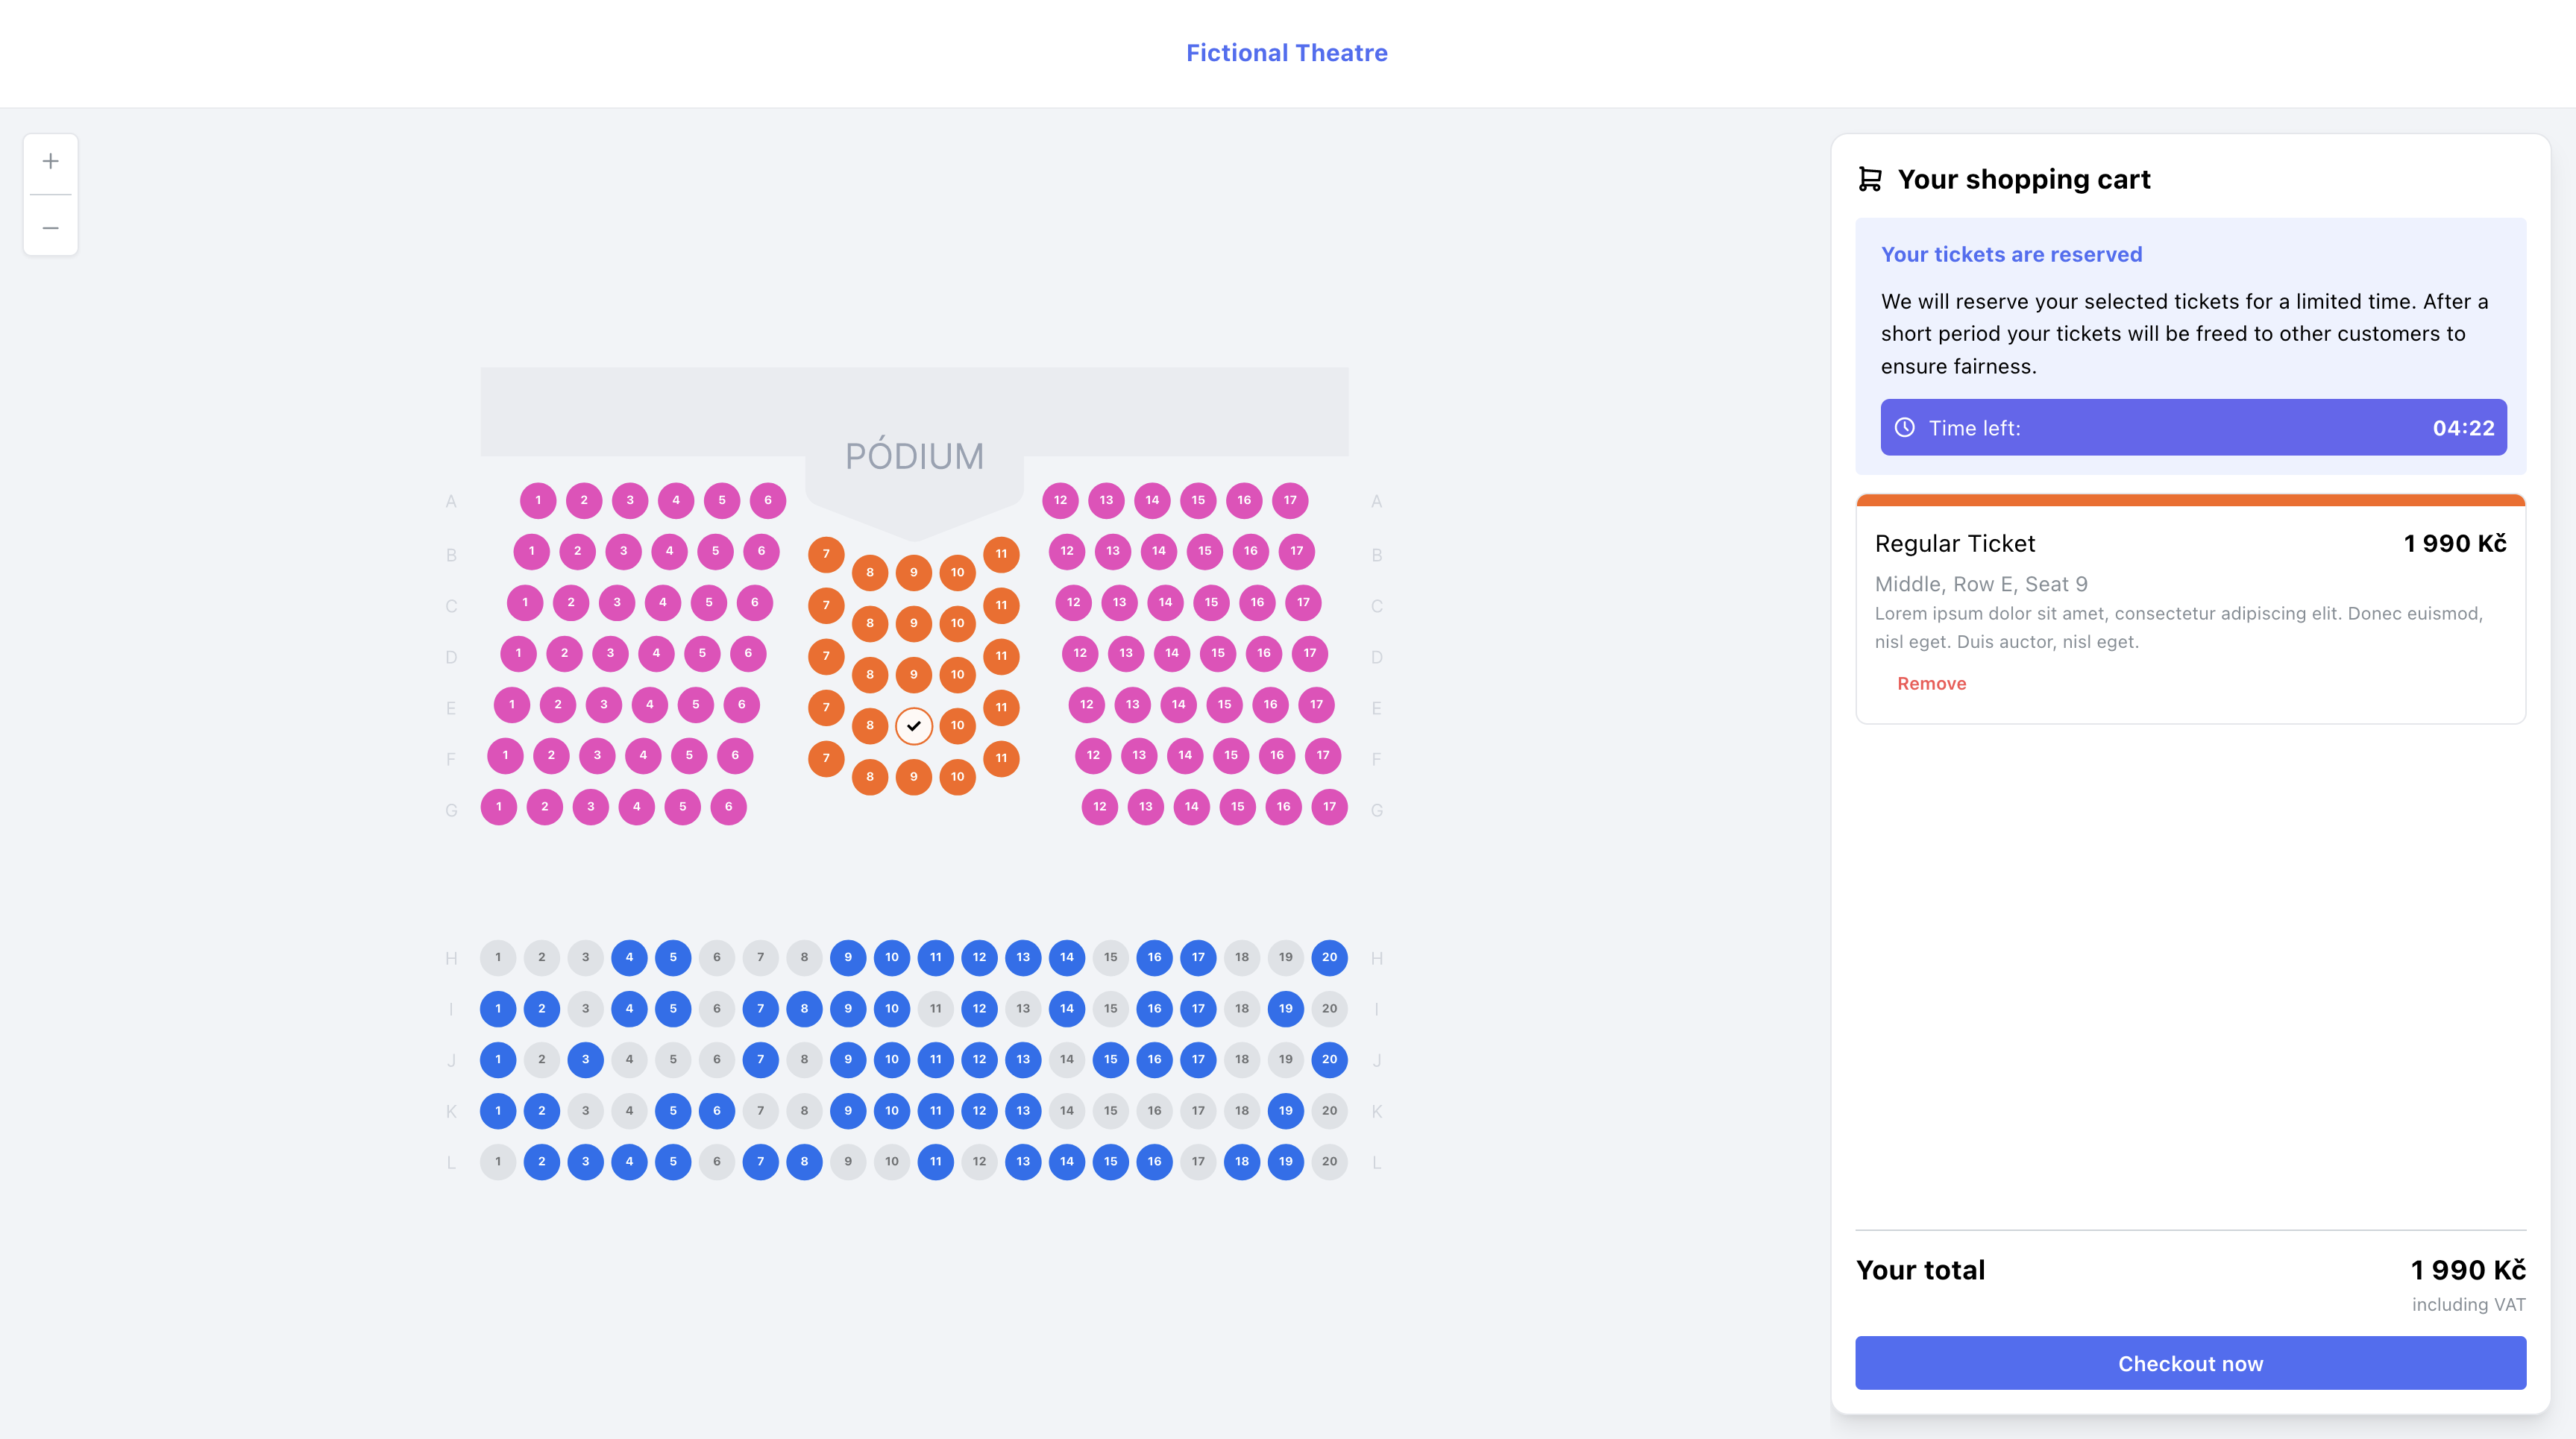
\includegraphics[width=\textwidth]{\FIGDIR/seating-map-cart}
	\caption{Snímek obrazovky košíku}
	\label{fig:seating-map-cart}
\end{figure}

%%% Podsekce – Integrace API
%%%%% Wording: ⏳
%%%%% Styling: ⏳
%%%%% References: ⏳
%%% --------------------------------------------------------------
\subsection{Integrace API}
\label{subsec:implementace-kosik-api}
State košíku je synchronizován s mock API, aby se napodobila situace v reálné aplikaci.
Kdykoli uživatel provede akci na košíku, je stav košíku aktualizován s malým zpožděním, aby se napodobila síťová latence reálného API.
Toho je dosaženo voláním asynchronní funkce, která vrací slib, který se vyřeší po nějaké době.
Funkce se nazývá \texttt{simulatedNetworkDelay} a je zobrazena v následujícím ukázce kódu spolu se všemi potřebnými podfunkcemi:

\begin{minted}{typescript}
/**
 * Simulates network delay
 * @param {"normal" | "heavy"} type
 * @return {Promise<void>}
 */
export const simulatedNetworkDelay = async (type: 'normal' | 'heavy' = 'normal') => {
	const delay = type === 'normal' ? 1000 : 5000;
	await fakePromise(DELAY_NETWORK ? randomIntBetween(delay * 0.25, delay) : 0);
};

/**
 * Resolves generated promise with optional value
 * @param {number} delay
 * @param {() => any} resolver
 * @param value
 * @returns {Promise<unknown>}
 */
export const fakePromise = (delay: number, resolver?: () => any, value?: any) =>
	new Promise((resolve) =>
		setTimeout(
			() => {
				resolver?.();
				resolve(value);
			},
			delay,
			value,
		),
	);

/**
 * Returns random integer from an interval
 * @param {number} min
 * @param {number} max
 * @return {number}
 */
export const randomIntBetween = (min: number, max: number): number => Math.floor(randomNumBetween(min, max));
\end{minted}

Užití funkce \texttt{simulatedNetworkDelay} je zobrazeno v následujícím ukázce kódu, která implementuje metodu \texttt{removeFromCartHandler}:

\begin{minted}[highlightlines={9-10}]{typescript}
/** remove from cart handler */
const removeFromCartHandler = useHandler<Types.UseCart.RemoveFromCartCb>(
	async (cartedTicketId) => {
		/** clear reservation if last carted ticket */
		if (cartedTickets.length === 1) {
			console.log('[Cart] Removing last carted ticket, removing reservation...');
			await simulatedNetworkDelay();
			await clearReservationHandler.handler();
		}
		/** TODO: API should be called instead */
		await simulatedNetworkDelay();
		console.log('[Cart] Updating reserved cart');
		/** remove from cart */
		console.log('[Cart] Removing from cart:', cartedTicketId);
		_setCartedTickets((prev) => prev.filter(({ cartedTicketId: _cartedTicketId }) => _cartedTicketId !== cartedTicketId));
	},
	{
		deps: [cartedTickets],
	},
);
\end{minted}

Detaily zmíněné výše jsou jádrem logiky košíku.
Jak se může zdát, logika košíku je poměrně jednoduchá, ale je zásadní pro funkčnost aplikace.
V kódu výše na řádku 9 je podmíněné volání \texttt{clearReservationHandler}, který je obslužným programem, který v případě odebrání poslední vstupenky z košíku vymaže rezervaci.
Více o rezervaci a jejím řízení je popsáno v následující sekci.
